\chapter{Graphics and tables}\label{sec:graphics}
Graphics files are inserted via the package \texttt{graphicx} which is
loaded in the document preamble (in file \texttt{report.tex}).
\par
Here we deal firstly with the inclusion of a single unlabelled diagram,
and then with captioned, labelled, and multiple diagrams.
\par
After that we consider tables of information.
%
\section{Plain}
Here is a colour \texttt{.jpg} file, inserted in place without caption
and without a number for cross-reference. It's suitable only for a
simple self-explanatory diagram, used here and not again.
\begin{center}
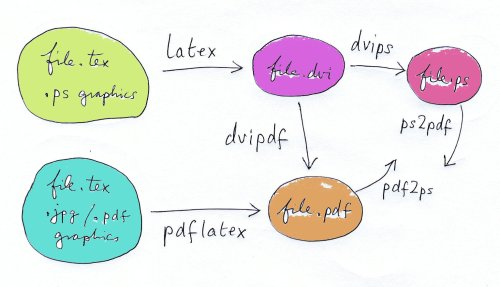
\includegraphics[width=.7\textwidth]{pic1.jpg}
%\includegraphics[width=.7\textwidth]{pic1new.jpg}
\end{center}
It shows the normal routes from a \LaTeX\ source (\texttt{.tex} file) to
\texttt{.ps} or \texttt{.pdf} output depending on the nature of the
graphics files included\footnote{An IDE such as TeXnicCenter has menu
buttons for each part of each route.}. \textit{Confusion over these
routes is a frequent source of grief}.
\par
This template has diagrams and graphs in \texttt{.jpg}
format\footnote{File extensions must be \texttt{.jpg} and not
\texttt{.JPG} or \texttt{.jpeg}.} and so its source is compiled to a
\texttt{.pdf} file with the command or menu button \texttt{pdflatex}.
\par
Mathematical software such as \textsl{Maple} and \textsl{Matlab} can
produce either \texttt{.ps} or \texttt{.jpg} diagrams, while cameras and
scanners\footnote{The figure itself is hand-drawn and scanned.} usually
produce \texttt{.jpg}. If accurate detail is vital, \texttt{.ps} is
best.
\par
With care, you can mix some graphics formats within a document. For
instance, if you compile to \texttt{.pdf} then you can use an
arbitrary mix of \texttt{.jpg}, \texttt{.png} and \texttt{.pdf}
graphics, but not \texttt{.ps}. And a document to be compiled to
\texttt{.dvi}, including \texttt{.ps} graphics, can include other
formats too if they are explicitly given \Quote{bounding boxes}. But
it's relatively tricky and you're better-off converting everything to
one format.
\par
Note that you can't include \texttt{.bmp} or \texttt{.gif} files at
all, but conversion of graphics files --- from \texttt{.bmp} to
\texttt{.jpg} for example --- is easily done with software like
\textsl{PhotoShop} \cite{PS} or \textsl{ImageMagick} \cite{IM}.
\par
It's simplest to keep your image files in the same directory as your
\texttt{.tex} files. Otherwise you can explore the mysteries of
\verb+\graphicspath+ \cite[Sec.~10.2.5]{MG}. In any case, use only
forward slashes in a directory specification. Names of directories and
of graphics files \textit{must not} include spaces!
%
\section{Fancy}
It's awkward to flow text round a picture, but it can be done with
packages such as \texttt{picinpar} or \texttt{wrapfig}, as \comp\
explains \cite[Sec.~6.4.1]{MG}.
\begin{center}
\begin{minipage}[c]{.45\textwidth}\centering
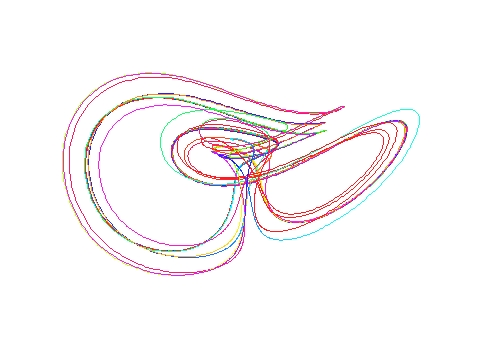
\includegraphics[width=.9\textwidth]{pic2.jpg}
\end{minipage}
\hfill\begin{minipage}[c]{.45\textwidth} And here's a \texttt{.jpg}
image side-by-side with some explanation, using the \texttt{minipage}
environment.\end{minipage}\end{center}
Something more elaborate sometimes gives unexpected results.
\par
\begin{figure}[ht]\centering
  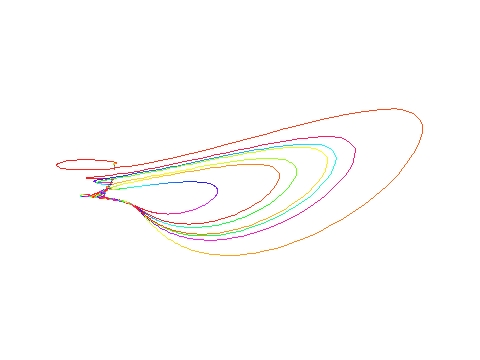
\includegraphics[width=.7\textwidth]{pic3.jpg}
  \caption{This is a caption explaining the diagram 
clearly and fully.}\label{fig:pic}
\end{figure}
That is, a picture \lq floating\rq\ in a \texttt{figure} environment
--- with a caption and number as in Fig.~\ref{fig:pic} --- might be
placed by \LaTeX\ on a page well after the text meant to accompany it.
\par
This happens if you have a relatively high density of graphics to
text. You may be able to deal with it by re-distributing the
pictures, changing the size of some of them, and the careful use of
paragraph breaks. Otherwise you may resort to \verb+\clearpage+,
which forces insertion of floating objects waiting to go in.
\par
The \nss\ book \cite{NSS} has Sec.~2.12 on the issue of \lq floating
bodies\rq\ and \comp\ has a whole chapter \cite[Chap.~6]{MG} on \lq
mastering floats'.
\par
Note that inside a \verb+figure+ (or \verb+table+) environment the 
\verb+\label+ must always {\em follow} the \verb+\caption+ --- see 
\cite[p.~67]{MG}.
\par
\begin{figure}[ht]\centering
\begin{minipage}[c]{.45\textwidth}\centering
  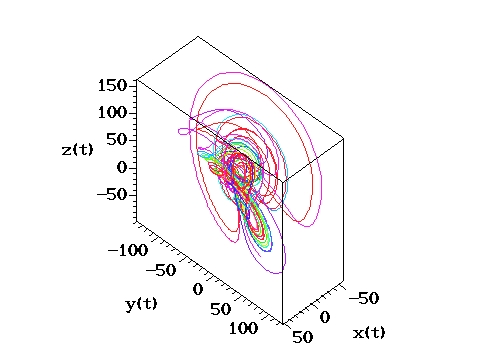
\includegraphics[width=.95\textwidth]{pic4.jpg}
  \caption{Caption to explain the diagram 
clearly and fully.}\label{fig:pictwo}
\end{minipage}\hfill
\begin{minipage}[c]{.45\textwidth}\centering
  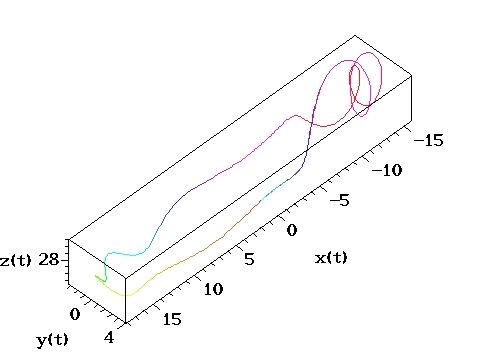
\includegraphics[width=.95\textwidth]{pic5.jpg}\\
  \caption{Caption to explain the diagram
clearly and fully.}\label{fig:picthree}
\end{minipage}
\end{figure}
Fig~\ref{fig:pictwo} and Fig.~\ref{fig:picthree} are two pictures
floating side-by-side, each in a \texttt{minipage} and each with its
own caption and label. This can be an economical way to insert multiple
diagrams.
\par
But don't get carried away and cram too many pictures together.
Be aware of the size-reduction that's often necessary, and maintain
legibility by choosing large enough font and weight for symbols,
axis-labels and other text.
\par
Figure captions should give plenty of information, because readers will
first skim the Introduction and Conclusions --- and then look at the
pictures. If you want (really really want) to hook them, make sure that
every important figure plus its caption is as self-explanatory as
possible.
%
\section{Tables}\label{sec:tables}
Besides figures you may want to include tables. Like figures, tables may
be plain and simple --- short and for immediate and local use only ---
and so put in place without a caption or label; or they may be
complicated and important enough to need a reference label and an
explanatory caption. Here are examples of each in turn.
\par
First a simple table \dots\par
\begin{center}
 \begin{tabular}{|l||c|c|c|r|}
    \hline
    row 1& it's & just & as & easy \\ \hline
    row 2& as & this & \(E=mc^2\) & what \\ \hline
    row 3& could & be & simpler & ? \\ \hline
    row 4& as & easy & as & \(\Pi\) \\ \hline
  \end{tabular}
\end{center}
\par
Here it is again, now floating in a \texttt{table} environment, with
a caption and a label to identify it as Table~\ref{table:one}.
\begin{table}[h]
  \centering
\begin{tabular}{|l||c|c|c|r|}
    \hline
    row 1& it's & just & as & easy \\ \hline
    row 2& as & this & \(E=mc^2\) & what \\ \hline
    row 3& could & be & simpler & ? \\ \hline
    row 4& as & easy & as & \(\Pi\) \\ \hline
  \end{tabular}
  \caption{Floating table, with a caption to explain it 
clearly and fully.}\label{table:one}
\end{table}
The remarks about giving full information in figures and their
captions apply equally to tables, of course. So do the remarks about
unexpected placement of floating objects.
\par
If you need a long table, occupying more than a page, and which
can't reasonably be divided, then you need to delve into \comp\
\cite[Chap~5]{MG} to find the secret.
%---------
\section{Summary}
Graphics files are evidently straightforward to include. If you need
to go beyond the basics, then refer to \Quote{The Graphics Companion}
\cite{GRM}.
\par
Tables are easy to use too, but don't misuse them. Lengthy data-sets can
be supplied separately on CDrom. Put only summaries in the report,
perhaps as an Appendix.
